\begin{figure}[h!]
  \vspace{-1em}
  \centering
  \def\figsep{.2cm}
  \def\dist{1}
  \def\disty{.9}
  \begin{subfigure}[b]{.24\textwidth}
    \subcaptionbox{Our approach with $\beta = 1$ \label{fig:cnr-2000-ab}}{%
      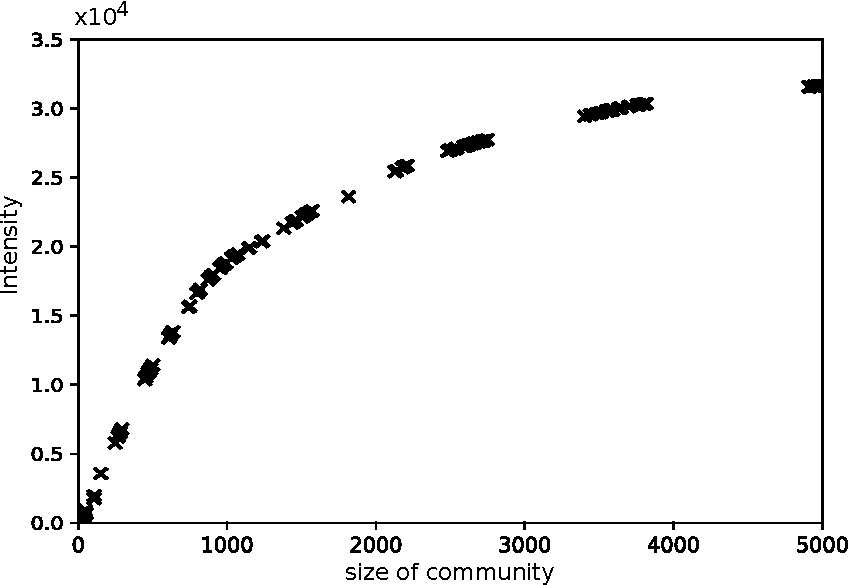
\includegraphics[width=\linewidth]{ab_cnr-2000.pdf}
    }
    % \label{fig:cnr-2000-ab}    
  \end{subfigure}
  \hfill
  \begin{subfigure}[b]{.24\textwidth}
    \subcaptionbox{SSM algorithm. (\cite{nagano2011size})\label{fig:cnr-2000-nagano}}{%
      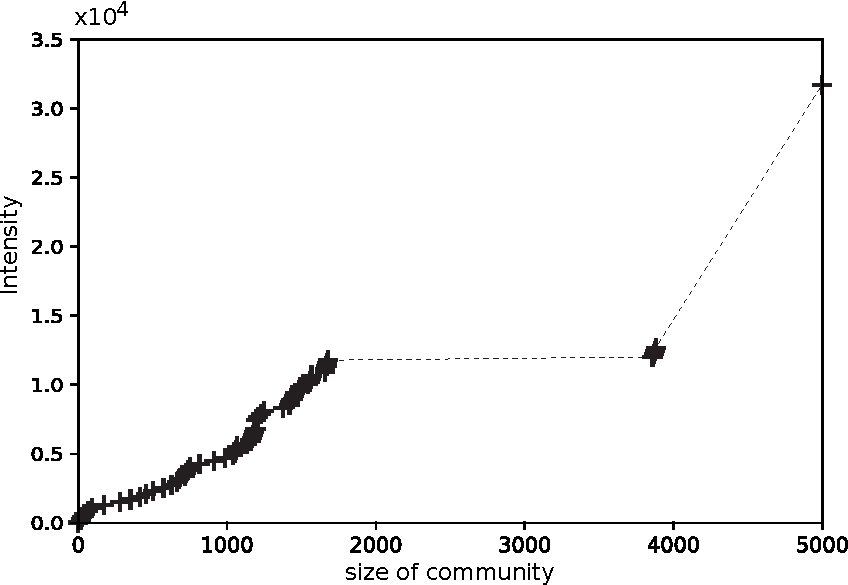
\includegraphics[width=\linewidth]{nagano_cnr-2000.pdf}
    }
    % \label{fig:cnr-2000-nagano}    
  \end{subfigure}
  \caption{Intensity (i.e., total weight of internal edges) versus the size (number of vertices) of
	  the subgraphs returned by (a) our approach and (b) by \cite{nagano2011size}.
	  %Our formulation returns more solutions (densest $k$-subgraphs) than 
	  %plots showing that the proposed algorithm discovers more densest subgraphts of
	  %large sizes. Our method retrieves 51 dense communities with cardinality $>$ 2000 while
	  %the SSM algorithm in \cite{nagano2011size} only finds 2 such communities.}
  }
  \label{fig:cnr-2000}
\end{figure}
